\scanpage{33}

\margin{hyp. de \unsure{induction}}
3°) L'hom can
\[
\diagram{\begin{tikzcd}
\Omega_X|Y \arrow[r] & \underline{\operatorname{Hom}}(\unsure{\varphi|\rho}_{Y/X},\Omega_Y)
\end{tikzcd}}
\]
est injectif [une orientation de X en $y\in Y$ est connue quand on sait comment \inserted{au vois. de y} une rive \inserted{de Y} détermine une orientation de Y]

\margin{\figure{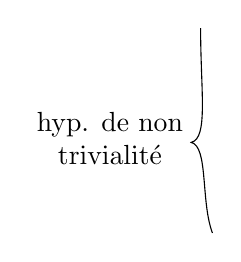
\begin{tikzpicture}[x=1cm,y=1cm]
\draw (0,2.6) .. controls (0,1.8) and (.1,1.2) .. (-.12,1.15) .. controls (.1,1.1) and (0,.4) .. (.15,0);
\node[left] at (-.1,1.2) {\shortstack{hyp. de non\\trivialité}};
\end{tikzpicture}}}
4°) Pour tte $\omega\in\unsure{\Gamma|\Omega}(X)$, l'hom correspondant
\[
\diagram{\begin{tikzcd}
\rho_{Y/X} \arrow[r] & \Omega_Y
\end{tikzcd}}
\]
est injectif [deux rives différentes définissent des orientations différentes de Y]

5°) Pour tout $X\in\operatorname{Ob}\mathcal V$, $\Omega(X)\to X$ est surjectif (il existe localement des orientations $\unsure{\omega|\varphi}$ de X; ou encore:
$\forall n\geq1$, $\Omega(\mathbb R^n)$ est non vide)

\margin{\figure{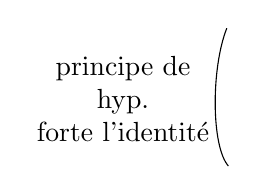
\begin{tikzpicture}[x=1cm,y=1cm]
\draw (.1,1.9) .. controls (-.1,1.4) and (-.1,.4) .. (.12,.15);
\node[left] at (0,1) {\shortstack{\inserted{principe de}\\\deleted{\unsure{hyp.}}\\\deleted{\unsure{forte}} \unsure{l'identité}}};
\end{tikzpicture}}}
6°) Pour tt $X\in\operatorname{Ob}\mathcal V$, $\Omega(X)$ interprété comme espace étalé sur X est séparé sur X, ou encore:
une orientation d'un $X\in\operatorname{Ob}\mathcal V$ est connue en un pt quand on la connaît en des pts arbitrairement voisins. (Il suffit de l'exiger pour $\mathbb R^n$, $n\geq1$, en fait, il sera vrai a posteriori qu'une orientation de $\mathbb R^n$, \inserted{ou de tt X connexe,} est connue quand on le connaît en un seul point\ldots)

\margin{32}
